\documentclass{standalone}
\usepackage{tikz}
\usepackage{amsmath}
\usepackage{pgfplots}

\begin{document}
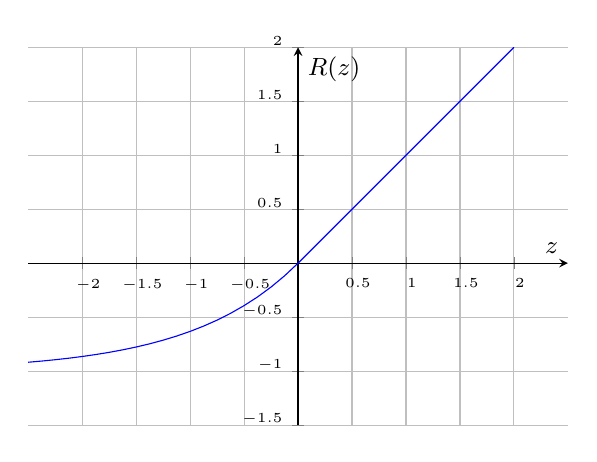
\begin{tikzpicture}[font=\small]

  \begin{axis} [
      unit vector ratio*=1 1 1,
        legend pos=north west,
            xmin=-2.5, xmax=2.5, ymin=-1.5, ymax=2, grid=both,
            ylabel={$R(z)$}, xlabel={$z$},
            xtick={-2,-1.5,...,2}, ytick={-2,-1.5,...,2},
            xticklabel style={font=\tiny, xshift=0.5ex},
            yticklabel style={font=\tiny, yshift=0.5ex},
            axis line style={->},
            axis x line=middle,
            axis y line=middle,
        ]
             
     
        \addplot+[mark=none, color=blue, domain=0:2] {x};
        \addplot+[mark=none, color=blue, domain=-3:0] {exp(x)-1};
        %   \addlegendentry[minimum height=4ex,text depth=1.5ex,font=\tiny]{$R(z)=
        %   \begin{cases} z & z < 0  \\
        %   \alpha (e^z–1) & z \geq 0 
        %     \end{cases}
        %     $
        %     }
        \end{axis}
        
        
        
    % \draw[->] (-3.5,0) -- (3.5,0) node[right] {$x$};
    % \draw[->] (0,-1.2) -- (0,3.5) node[above] {$f(x)$};
    % \draw[scale=1,domain=0:3,smooth,variable=\x,blue] plot ({\x},{\x});
    % \draw[scale=1,domain=-3:0,smooth,variable=\x,blue] plot ({\x},{exp(\x)-1});
    % \draw[dashed, scale=1,domain=-3.2:3.2,smooth,variable=\x,blue] plot ({\x},{-1});
\end{tikzpicture}
\end{document}

